\documentclass[12pt]{article}
\usepackage{sbc-template}
\usepackage{graphicx,url,float}
\usepackage{hyperref}
\usepackage[alf]{abntex2cite}
\usepackage[brazil]{babel}   
\usepackage[utf8]{inputenc} 
     
\sloppy

\title{Azure CosmosDB: Estudo e aplicação}

\author{Athos Castro Moreno}

\address{Departamento de Computação - Universidade Tecnológica Federal do Paraná
  (UTFPR)\\
  Avenida Alberto Carazzai, 1640 -- 86300000 -- Cornélio Procópio -- PR -- Brasil
  \email{athos@alunos.utfpr.edu.br}
}

\begin{document} 

\maketitle

\begin{resumo} 
	O Azure CosmosDB é um serviço de banco de dados NoSQL auto-gerenciável disponível na rede da Azure para utilização para o público. Este artigo é destinado para explorar as possibilidades
	do serviço, suas funcionalidades como um banco de dados distribuído e como utilizar. 
\end{resumo}

\section{Introdução}
Na indústria de tecnologia de informação é comum a utilização dos bancos de dados relacionais que usufruem da linguagem SQL para as operações. Com a crescente demanda
de maleabilidade na modelagem de um banco de dados em empresas com requisitos que não estão com uma estrutura de dados bem definida, precisam de um desenvolvimento mais rápido
ou estão em constante mudança foi necessária a utilização de soluções além de bancos de dados relacionais \cite{Oliveira2011}.

Para alguns casos, utilizar um banco de dados não relacional resolve algumas das dificuldades de um banco de dados relacional. Também chamado de NoSQL (\textit{Not Only SQL}),
possui diversas implementações no mercado -- a grande maioria, \textit{open source} -- voltadas a algum problema especifico \cite{Pokorny2013}.

\section{NoSQL}
O conceito de bancos de dados não relacionais existe desde 1960 e ganhou popularidade entre 2007 e 2010, principalmente com o anúncio do Amazon Dynamo, serviço de uso interno no \textit{e-commerce}
da Amazon, que posteriormente se tornou a base do AWS DynamoDB, serviço NoSQL disponível para uso na Amazon Web Services \cite{DeCandia2007}.
A primeira implementação NoSQL foi criada por Carlo Stozzi, aonde um banco de dados \textit{open source} em shell não utilizava nenhuma interface SQL para ser manipulado \cite{Lith2010}. 

Cada implementação NoSQL possuí uma abordagem diferente, tais como \cite{Lith2010} \cite{Leavitt2010}:

\begin{itemize}
	\item \textbf{\textit{Key-value}:} Armazena um par de chaves e valores, funcionando com um \textit{array} associativo. Pode armazenar dados estruturados ou dados sem estrutura.
	\item \textbf{Orientado a documentos:} Uma subclasse do \textit{key-value}, tendo diferença no processamento dos dados através da estrutura interna do documento. Podem ser utilizados 
	os formatos de arquivos XML, YAML, JSON, BSON, entre outras opções.
	\item \textbf{Orientado a colunas:} Nessa abordagem as informações são armazenadas em colunas. É otimizado para recuperação rápida de dados, uso em aplicativos 
	analíticos e reduz requerimentos de E/S de disco e quantidade de dados necessário a serem carregados.
\end{itemize}

O uso de um banco de dados NoSQL é recomendado para ambientes dinâmicos, que precisem ser escaláveis entre várias máquinas de maneira mais rápida, com uma estrutura de dados que não está bem 
definida ou em constante mudança. É importante ressaltar que o NoSQL não tem como foco substituir todos os bancos relacionais existentes e sim fornecer uma alternativa para os que 
precisam de mais velocidade e estar menos presos a uma modelagem \cite{Oliveira2011} \cite{Lith2010} \cite{Leavitt2010}. 

\section{Azure CosmosDB}
O produto CosmosDB iniciou em 2010 como um projeto interno na Microsoft, conhecido como Projeto Florence. O objetivo do projeto era resolver problemas de desenvolvimento em aplicações de Internet
que eram utilizadas em larga escala, similar a razão da Amazon ter criado o Dynamo. Em 2015 o projeto foi disponibilizado para usuários do Azure com o nome de DocumentDB. Em 2017, no evento Build 2017,
o DocumentDB foi lançado com o nome de CosmosDB com as funcionalidades já existentes, mais a distribuição global presente hoje \cite{Paz2018}.

Além das vantagens do NoSQL, o CosmosDB fornece outras funcionalidades. A mais importante é a georeplicação via portal nos \textit{datacenters} da Azure e além desta, tem baixa latência de leitura/escrita,
serviço auto-gerenciado -- não é necessário atualizar ou modificar nenhum \textit{software}, suporta múltiplos \textit{data models}, escalabilidade de custo e \textit{failover} automático, se configurado \cite{Paz2018} \cite{Shukla2015}.

É importante lembrar que o CosmosDB, apesar de utilizar e suportar diversas tecnologias \textit{open source}, é um serviço proprietário da Microsoft e seu uso é limitado dentro dos 
servidores da Azure.

\subsection{Modelos de Consistência}
O CosmosDB possui cinco modelos de consistência que podem ser escolhidos de acordo com a necessidade do aplicativo em que será usado. Cada modelo de consistência possui vantagens, desvantagens e limitações.
É possível entre \cite{Paz2018} \cite{Shukla2015}:

\begin{itemize}
	\item \textbf{\textit{Strong Consistency:}} Garante que toda leitura de um item irá retornar a versão mais recente deste item e o usuário nunca irá ver uma versão incompleta do item. 
	É o mesmo modelo de consistência existente em bancos de dados relacionais, por isso o CosmosDB não permite que quando o modelo \textit{strong consistency} está configurado, não é possível utilizar a funcionalidade
	de replicação global.
	\item \textbf{\textit{Eventual Consistency:}} Garante que eventualmente, todas as replicas irão, eventualmente, convergir para refletir a escrita mais recente. Em termos de consistência de dados é um modelo fraco, mas,
	oferece a menor latência de todos os modelos oferecidos. 
	\item \textbf{\textit{Bound Staleness Consistency Model:}} Neste modo é possível afirmar que as leituras irão atrasar entre as escritas por um numero \textit{K} de operações ou em um intervalo \textit{t} de tempo. O valor \textit{K} deve estar entre
	10 e 1000000 operações ou entre 100000 e 1000000 se o banco é globalmente distribuído. O valor \textit{t} pode ser entre cinco segundos e um dia ou cinco minutos e um dia para bancos distribuídos globalmente.
	\item \textbf{\textit{Session Consistency Model:}} O nível de consistência é definido na sessão do cliente. Todas as leituras e escritas estão sempre atualizadas dentro da mesma sessão, durante seu tempo de vida. Esse modelo fornece uma
	alta taxa de transferência e baixas taxas de latência de escrita e é o modo padrão para toda conta nova do CosmosDB. 
	\item \textbf{\textit{Consistent Prefix Consistency Model:}} Similar ao modelo anterior, garante que as leituras nunca irão ver escritas fora de ordem. 
\end{itemize}

\subsection{APIs disponíveis}
É possível utilizar o CosmosDB com cinco APIs diferentes:
\begin{itemize}
	\item \textbf{SQL:} O CosmosDB fornece uma API que suporta \textit{queries} em linguagem SQL em um banco de dados JSON não relacional. Apesar de utilizar SQL, não são suportadas \textit{queries} de junção.
	\item \textbf{MongoDB:} O MongoDB é um banco de dados NoSQL conhecido e estabelecido no mercado. O CosmosDB suporta a utilização de bancos de dados no MongoDB, podendo utilizar \textit{drivers} existentes e importar bancos já criados
	em outras instâncias.
	\item \textbf{Graph:} É possível criar um banco de dados baseado em grafos NoSQL, com suporte a API do Gremlin, uma linguagem para manipulação de bancos de dados em grafos.
	\item \textbf{Tabelas:} É possível portar tabelas criadas no serviço Azure Table para o CosmosDB sem nenhuma modificação no código.
	\item \textbf{Cassandra:} É possível criar bancos de dados NoSQL com o Apache Cassandra, outro banco de dados \textit{open-source} estabelecido no mercado.
\end{itemize}

\subsection{Como utilizar}
O CosmosDB é um serviço pago da Azure, sendo necessário criar uma conta na Azure para utilizar. Para usuários novos, a Azure fornece um ano de serviços selecionados de uso gratuito, incluindo o CosmosDB. É necessário possuir um cartão de crédito
para ativar a conta da Azure e utilizar os serviços no período gratuito. As figuras 1 e 2 mostram o processo de criação de um banco de dados MongoDB novo no CosmosDB. A figura 3 mostra o mapa de 
georeplicação no portal da Azure. A figura 4 mostra os modos de consistência para serem escolhidos no portal da Azure.

\begin{figure}[H]
	\label{fig:az1}
	\caption{Criação do banco de dados CosmosDB} 
	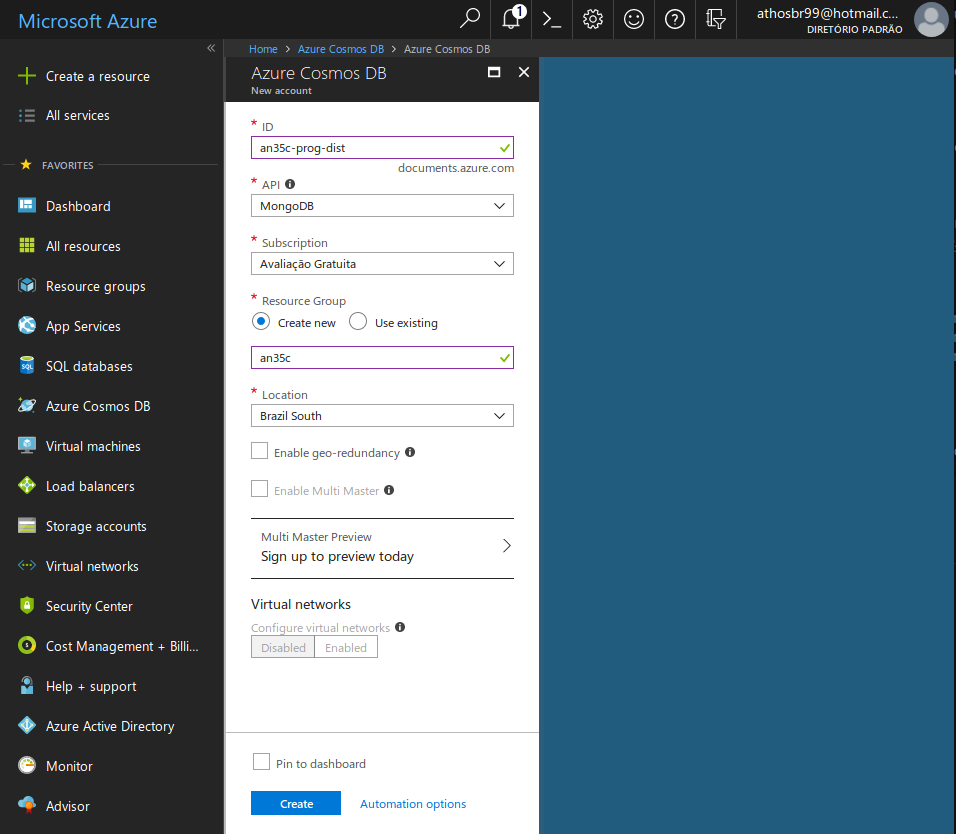
\includegraphics[scale=0.27]{img/az1.png}
	\centering
\end{figure}

\begin{figure}[H]
	\label{fig:az2}
	\caption{Esperando o processo terminar a criação da instância}
	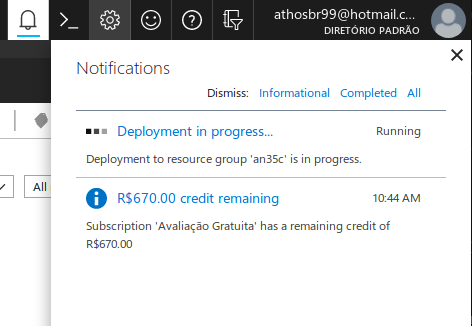
\includegraphics[scale=0.27]{img/az2.png}
	\centering
\end{figure}

\begin{figure}[H]
	\label{fig:az4}
	\caption{Mapa de georeplicação}
	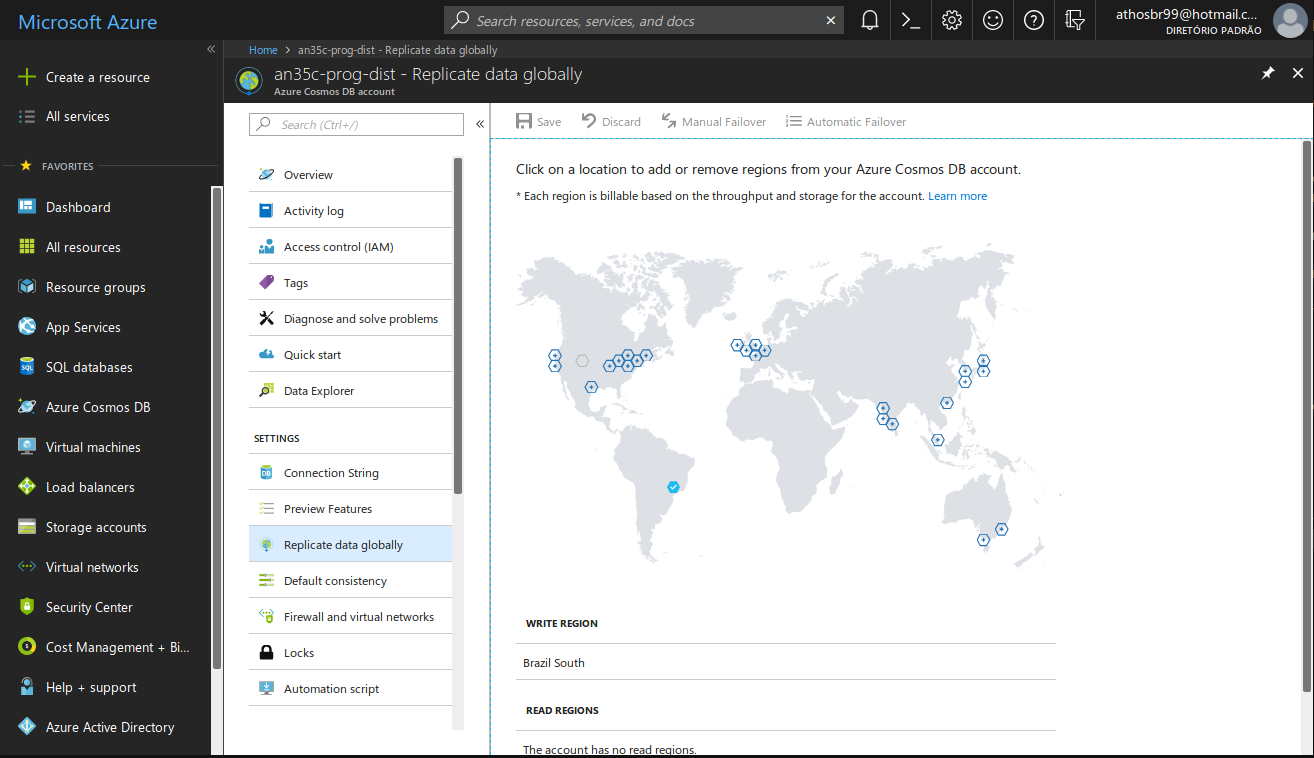
\includegraphics[scale=0.27]{img/az4.png}
	\centering
\end{figure}

\begin{figure}[H]
	\label{fig:az5}
	\caption{Modos de consistência}
	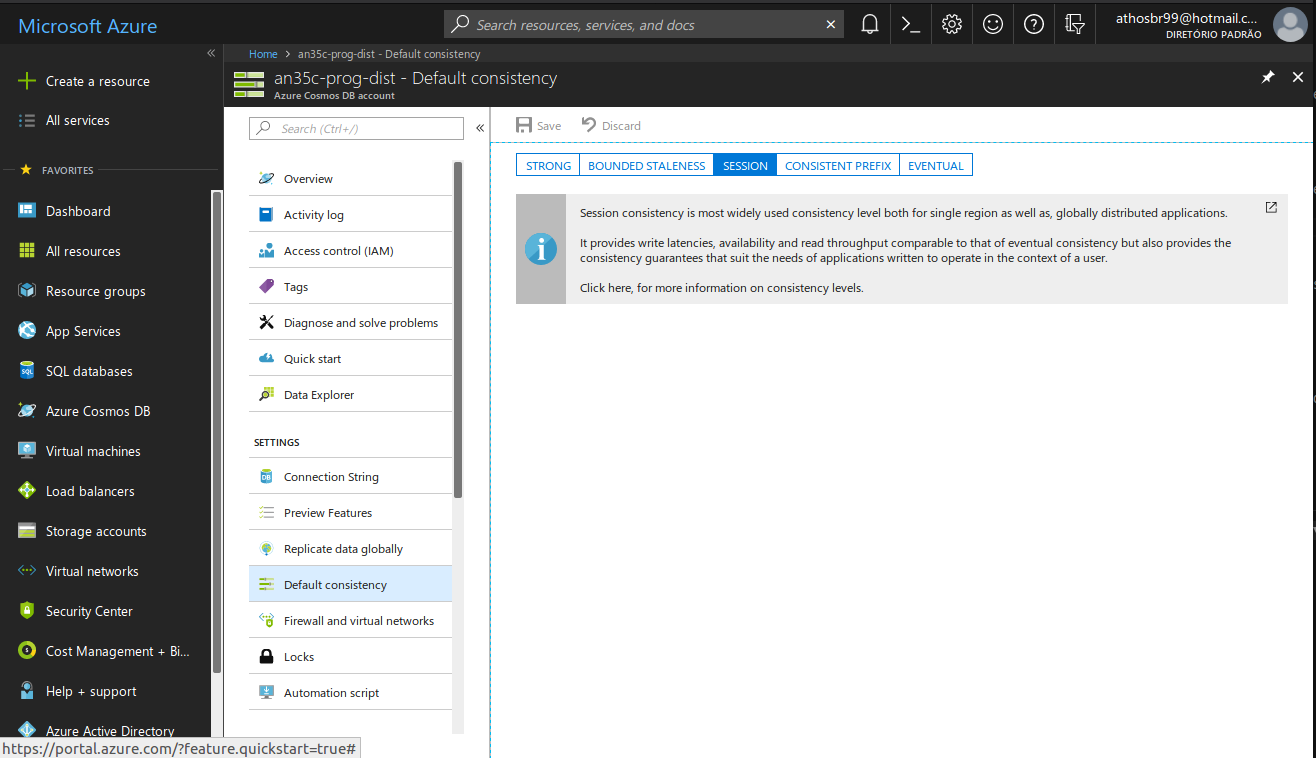
\includegraphics[scale=0.27]{img/az5.png}
	\centering
\end{figure}

\subsection{Modelo de cobrança}
O CosmosDB utiliza o conceito de \textit{Request Units} -- traduzido como unidades de solicitação -- para a cobrança do serviço. Esse número abstrai recursos físicos necessários para as requisições, é 
determinístico por operação e são isolados por região, significando que caso um servidor esteja replicado em mais de uma região, cada leitura por região irá exigir suas próprias unidades de requisição.
Cada requisição exige uma quantidade de unidade de solicitação que é baseada na quantidade computacional necessária para executar a solicitação.

É possível utilizar o website \url{https://www.documentdb.com/capacityplanner} para estimar quanto será gasto em unidades de solicitação para processar um arquivo JSON. Um exemplo de calculo é mostrado na
Figura 5. O exemplo utilizado foi retirado da página \url{https://www.json.org/example.html}.

\begin{figure}[H]
	\label{fig:az6}
	\caption{Estimativa de uso de unidades de solicitação}
	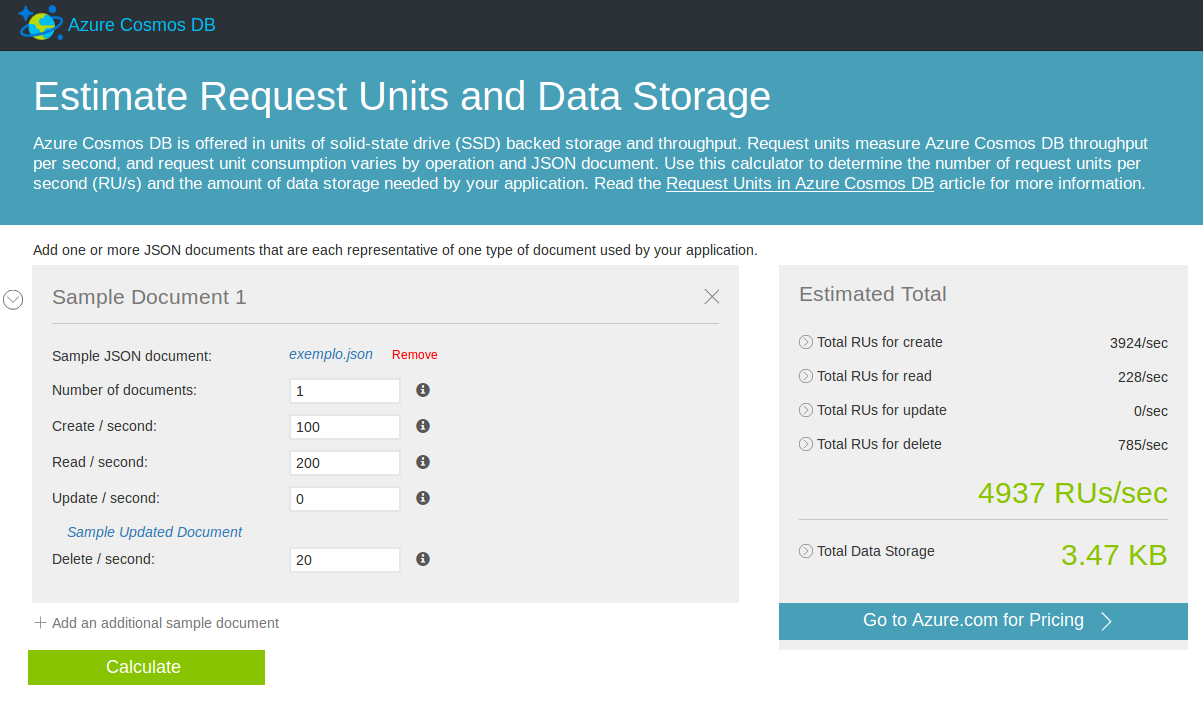
\includegraphics[scale=0.27]{img/az6.png}
	\centering
\end{figure}

\subsection{Concorrentes}
Os concorrentes diretos do Azure CosmosDB são o BigTable (Google Cloud Platform), DynamoDB (Amazon Web Services) e AosaraDB (Alibaba Cloud). Apesar de todos serem bancos de dados NoSQL autogerenciaveis, apenas o AWS DynamoDB fornece replicação 
global que também é disponível no CosmosDB. Nenhum dos concorrentes citados fornece acesso a multíplas APIs igual é fornecido no Azure CosmosDB.

\section{Exemplo prático}
Um exemplo prático foi feito para demonstrar o funcionamento do CosmosDB. A prova de conceito foi feita utilizando JavaServer Faces com o propósito de mostrar que é possível utilizar o serviço em tecnologias consideradas mais antigas. Instruções e imagens podem
ser encontradas no repositório \url{https://github.com/athosbr99/an36a-cosmosdb}.

\section{Conclusão}
O Azure CosmosDB é um serviço para quem precisa de um banco de dados NoSQL autogerenciado e com capacidade de replicação que seja prático de ser utilizado, além da possibilidade de utilizar diversas implementações NoSQL disponíveis. Porém, seu preço e curva de
aprendizado pode ser proibitivo para times com pouco orçamento, curto prazo de entrega ou com poucos profissionais experientes. Outro fator que pode influenciar a decisão é a obrigatoriedade de utilizar a infraestrutura da Microsoft, que em alguns casos é um incentivo devido a abstração fornecida pelo
Azure e em outros casos pode ser um impeditivo, seja por regras de \textit{compliance} ou politicas internas de uma empresa. 

\bibliography{bibliografia}

\end{document}